% ======================================================================
%  BIBM / IEEE 课程论文模板（支持中英文混排）
%  适用课程：《生物文本挖掘与知识发现》等
%  编译方式：pdflatex  ->  bibtex  ->  pdflatex  ->  pdflatex
%  依赖宏包：IEEEtran.cls（BIBM 官方模板，请与本文件放同一目录）
% ======================================================================
\documentclass[conference]{IEEEtran}
\IEEEoverridecommandlockouts

% ---------- 基础宏包 ----------
\usepackage{cite}
\usepackage{amsmath,amssymb,amsfonts}
\usepackage{algorithmic}
\usepackage{graphicx}
\usepackage{textcomp}
\usepackage{xcolor}
\usepackage{url}
\usepackage{booktabs}   % 更漂亮的三线表（可选）

% ---------- 页码设置 ----------
% IEEE 模板默认不显示页码；通过 fancyhdr 在页脚居中显示页码。
\usepackage{fancyhdr}
\pagestyle{fancy}
\fancyhf{}                    % 清空默认页眉页脚
\fancyfoot[C]{\thepage}       % 页脚居中显示页码
\renewcommand{\headrulewidth}{0pt}  % 去掉页眉横线
\renewcommand{\footrulewidth}{0pt}  % 去掉页脚横线

% ---------- 页脚左下角灰色水印 ----------
% 课程论文声明：Agent 生成内容提示，灰色小字，左下角紧凑三行。
% 若不需要，注释掉下面 \fancyfoot[L]{...} 整段即可。
\fancyfoot[L]{%
  \scriptsize\color{gray}%
  \begin{tabular}[b]{@{}l@{}}
    课程论文支持使用 Agent 生成内容，\\
    这只是起点。人工内容审查\\
    和驾驭才是终点。%
  \end{tabular}%
}
\setlength{\footskip}{24pt}   % 给页脚留出足够空间，避免与正文重叠

% IEEEtran 的首页 (\maketitle) 默认使用 plain 样式，会覆盖上面的 fancy 设置。
% 这里把 plain 和 IEEE 标题页样式也改成同样的页脚，保证首页同样显示页码和水印。
\fancypagestyle{plain}{%
  \fancyhf{}%
  \fancyfoot[C]{\thepage}%
  \fancyfoot[L]{%
    \scriptsize\color{gray}%
    \begin{tabular}[b]{@{}l@{}}
      课程论文支持使用 Agent 生成内容，\\
      这只是开始。人工内容审查\\
      和驾驭才是终点。%
    \end{tabular}%
  }%
  \renewcommand{\headrulewidth}{0pt}%
  \renewcommand{\footrulewidth}{0pt}%
}
\fancypagestyle{IEEEtitlepagestyle}{%
  \fancyhf{}%
  \fancyfoot[C]{\thepage}%
  \fancyfoot[L]{%
    \scriptsize\color{gray}%
    \begin{tabular}[b]{@{}l@{}}
      课程论文支持使用 Agent 生成内容，\\
      这只是开始。人工内容审查\\
      和驾驭才是终点。%
    \end{tabular}%
  }%
  \renewcommand{\headrulewidth}{0pt}%
  \renewcommand{\footrulewidth}{0pt}%
}

% ---------- 行号设置 ----------
% 在页面左侧显示行号，方便老师批改/审稿时定位。
% 若提交最终版不需要行号，注释掉 \pagewiselinenumbers 一行即可。
\usepackage[switch]{lineno}   % switch: 双栏时行号显示在外侧
\pagewiselinenumbers          % 每页行号从 1 重新开始（也可改用 \linenumbers 全文连续编号）

% ---------- 中文支持（pdflatex 下也能用） ----------
% 说明：
%   1) 使用 ctex 宏包并开启 UTF8，即可在 pdflatex 下输入中文；
%   2) 缺少 Windows 中文字体时，先查询系统字体；使用 XeLaTeX 和 fontspec
%      自定义字体的方法见本目录 README。pdfLaTeX 需要匹配的 TeX 字体支持。
\usepackage[UTF8]{ctex}

\def\BibTeX{{\rm B\kern-.05em{\sc i\kern-.025em b}\kern-.08em
    T\kern-.1667em\lower.7ex\hbox{E}\kern-.125emX}}

\begin{document}

% ======================================================================
%  标题 / 作者 / 单位  ——  按需修改
% ======================================================================
\title{在这里填写论文标题\\
\large 副标题（可选，可写中文）}

\author{
\IEEEauthorblockN{姓名 (Your Name)}
\IEEEauthorblockA{
\textit{学号 } \\
\textit{专业或班级}
邮箱: your.email@example.com}
}

\maketitle

% ======================================================================
%  摘要 / 关键词
% ======================================================================
\begin{abstract}
% TODO: 在此填写摘要（150--250 字）
\end{abstract}

\begin{IEEEkeywords}
% TODO: 关键词1, 关键词2, keyword3, keyword4
\end{IEEEkeywords}

% ======================================================================
%  I. 引言
% ======================================================================
\section{引言 Introduction}
% TODO: 在此撰写引言（研究背景、问题定义、本文贡献列表）

% ======================================================================
%  II. 相关工作
% ======================================================================
\section{相关工作 Related Work}
% TODO: 在此撰写相关工作
% 示例：引用 reference.bib 中的文献
例如，Cancer-Alterome~\cite{canceralterome2024} 是一个文献挖掘资源；
NLTK~\cite{nltk2009} 是常用的自然语言处理工具；
本课程方法基于讲义~\cite{slides2026}；
信息检索的经典教材见~\cite{manning2008ir}。

% ======================================================================
%  III. 数据与方法
% ======================================================================
\section{数据与方法 Data and Methods}
\subsection{数据 Data}
% TODO: 描述数据来源、规模、字段

\subsection{预处理 Preprocessing}
% TODO: 说明分词、大小写、停用词、别名归一化等决策

\subsection{方法 Methods}
% TODO: 写下方法公式

% ======================================================================
%  IV. 结果
% ======================================================================
\section{结果 Results}
\subsection{整体统计 Overall Statistics}
% TODO: 给出数据分布图或表

% ---------- 示例：插入图片（figure/fig_example.pdf） ----------
% 图片文件放在 figure/ 子目录中，引用时使用相对路径 figure/fig_example.pdf
% 在正文中用 "如图~\ref{fig:example} 所示" 引用本图
\begin{figure}[h]
  \centering
  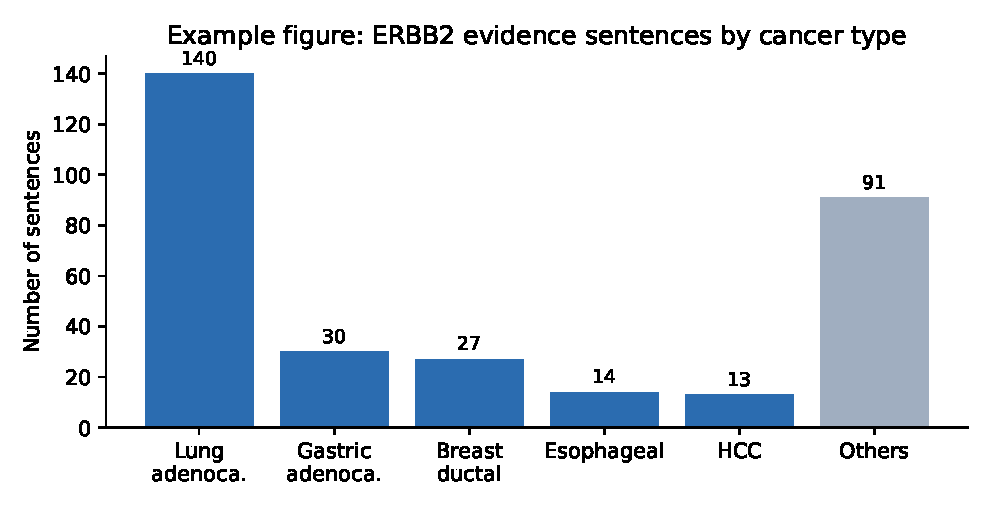
\includegraphics[width=\columnwidth]{figure/fig_example.pdf}
  \caption{示例图：不同癌症类型中 ERBB2 证据句子的分布（数据为示意）。
           Example bar chart of ERBB2 evidence sentences across cancer types.}
  \label{fig:example}
\end{figure}

如图~\ref{fig:example} 所示，肺腺癌的 ERBB2 证据句子数最多，
其余癌症类型依次递减。% TODO: 替换为你自己的图和描述

% ---------- 示例：三线表（booktabs） ----------
\begin{table}[h]
  \centering
  \caption{示例表格：不同癌症类型的 ERBB2 句子分布（数据为示意）。}
  \label{tab:example}
  \begin{tabular}{lrr}
    \toprule
    癌症类型 & 句子数 & 占比 (\%) \\
    \midrule
    肺腺癌 (Lung adenocarcinoma) & 140 & 44.4 \\
    胃腺癌 (Gastric adenocarcinoma) & 30 & 9.5 \\
    乳腺导管癌 (Breast ductal carcinoma) & 27 & 8.6 \\
    食管癌 (Esophageal carcinoma) & 14 & 4.4 \\
    肝细胞癌 (Hepatocellular carcinoma) & 13 & 4.1 \\
    其他 & 91 & 28.9 \\
    \midrule
    总计 & 315 & 100.0 \\
    \bottomrule
  \end{tabular}
\end{table}
% 用法：在正文中用 "见表~\ref{tab:example}" 引用本表

\subsection{主要发现 Main Findings}
% TODO: 逐条陈述主要发现

% ======================================================================
%  V. 讨论
% ======================================================================
\section{讨论 Discussion}
\subsection{结果意味着什么 Implications}
% TODO: 说明这些结果能支撑什么科学发现或结论

\subsection{局限性 Limitations}
% TODO: 诚实说明方法/数据的局限

\subsection{下一步 Future Work}
% TODO: 指出可以改进的方向

% ======================================================================
%  VI. 结论
% ======================================================================
\section{结论 Conclusion}
% TODO: 用一段话总结全文

% ======================================================================
%  致谢
% ======================================================================
\section*{Acknowledgment 致谢}
% TODO: 感谢导师、同学、课程、数据来源等

% ======================================================================
%  参考文献（使用 BibTeX，引用 reference.bib）
%  编译顺序：pdflatex -> bibtex -> pdflatex -> pdflatex
%  若你想改用手工 thebibliography，删除下面两行并自行添加条目即可。
% ======================================================================
\bibliographystyle{IEEEtran}
\bibliography{reference}   % 对应 reference.bib

\end{document}
